\chapter{Methodology}
\label{chap:framework}
First, we introduce in this chapter a lifelong learning approach for Dynamic Neural Networks~\cite{yoon2017lifelong}, which is a way to achieve simultaneous and effective multitasking by dynamically extending the neural network structure. Then our proposed framework based on the DEN model is described in detail.


\section{Related Work}\label{sec:related-4}

Lifetime learning, i.e., the problem of continuous learning where tasks arrive sequentially, is an important topic in transfer learning. The main goal of lifelong learning is to exploit the knowledge from earlier tasks to obtain better performance or to obtain faster convergence/training speed on the model for later tasks, but without forgetting the previous knowledge, i.e., the model parameters apply to the previous model.

Regarding lifelong learning, there are also many different approaches to implementation. The simplest approach is to gradually fine-tune the network to fit the new task by continuing to train the network with new training data. However, this simple retraining of the network can degrade the performance of both the new task and the old task. If the new task is very different from the old task, then the model trained for the new task, changes so much that it is no longer applicable to the old task. For example, the lifelong learning approach using  Elastic Weight Consoliation(EWC)~\cite{kirkpatrick2017overcoming} is as follows:
\begin{figure}[H]
	\centering
	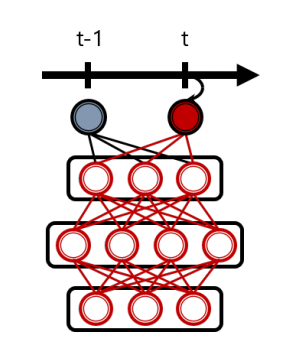
\includegraphics[width=1\linewidth]{figures_ning/ewc}
	\caption[Retraining w/o expansion]{Retraining w/o expansion}
	\label{fig:ewc}
\end{figure}
Elastic Weight Consoliation retrains the entire network learned in the previous task, while regularizing it to prevent large deviations from the original model. Units and weights in red indicate retrained units and weights, while black indicates units and weights that remain fixed.

The use of the EWC approach, i.e., limiting the weights, leads to smaller changes in the parameters, thus allowing the model trained for the new task to also be valid for the old task at the same time.

Of course, the disadvantage of this approach is also obvious. When the difference between the old and new tasks is large, it is difficult to make the model valid for the new task no matter how it is trained, because the elasticity limits the model parameters.

In addition to this there is a lifelong learning approach, fixed extension neural networks~\cite{rusu2016progressive}. For a new task, the original model parameters are no longer retrained, and a fixed number of neurons are directly expanded on the original neural network structure. In the subsequent training, only the newly added neurons are trained, and no further changes are made to the previous model parameters.
\begin{figure}[H]
	\centering
	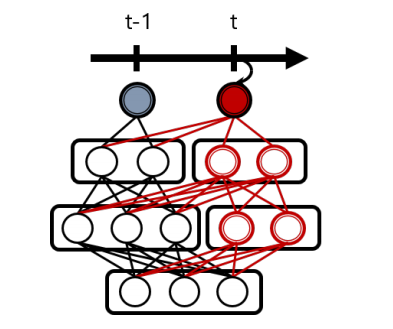
\includegraphics[width=1\linewidth]{figures_ning/no-train}
	\caption[No-retraining w/ expansion]{No-retraining w/ expansion}
	\label{fig:no-train}
\end{figure}
Units and weights colored in red denote the ones that are retrained, and black ones are ones that remain
fixed.

The disadvantage of this approach is also obvious, it is difficult to have an effect on the new task by the newly added part of neurons, because there are too few parameters that can be changed, or the previous parameters are too important.

However for such incremental deep learning setups with selective parameter sharing and dynamic layer scaling, many challenges need to be addressed.
\begin{enumerate}[\qquad  1.]
	\item Achieving scalability and efficiency in training: If the network capacity grows, the training cost per task will also get higher, as later tasks will establish connections to larger networks. Therefore, we need a way to keep the computational overhead of retraining low.
	\item Decide when to scale the network and how many neurons to add: If the old network adequately explains the new task, the network may not need to scale its size. On the other hand, if the task is very different from the existing one, it may need to add many neurons. Therefore, the model needs to dynamically add only the necessary number of neurons.
	\item prevent semantic drift or catastrophic forgetting, where the network deviates from its initial configuration during training, thus showing degraded performance of earlier examples/tasks. Since our approach retrains the network, even partially, to adapt to later learned tasks and adds new neurons that may also negatively affect previous tasks by establishing connections to older sub-networks, we need a mechanism to prevent potential semantic drift.
\end{enumerate}

To overcome these challenges, we propose a novel deep network model and an efficient and effective incremental learning algorithm, which we name as Dynamically Extensible Network (DEN). In a lifelong learning scenario, DEN maximizes the network learned on all previous tasks to efficiently learn to predict new tasks, while dynamically increasing the network capacity by adding or splitting neurons when necessary.

DEN solves the challenge presented above very well, since we retrain the network on each task t so that each new task only utilizes and changes relevant parts of the previously trained network, while still allowing to extend the network capacity if necessary. In this way, each task t will use a different sub-network from the previous task while still sharing a significant portion of the sub-network with them. As shown in the figure below:
\begin{figure}[H]
	\centering
	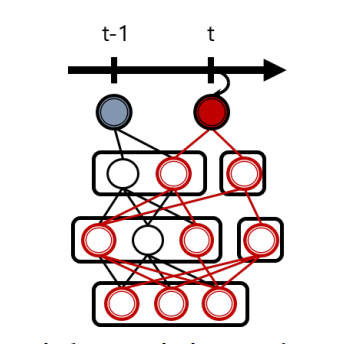
\includegraphics[width=1\linewidth]{figures_ning/den}
	\caption[Partial retraining w/ expansion]{Partial retraining w/ expansion}
	\label{fig:den}
\end{figure}

The advantages of the DEN method are also obvious, as more parameters can be changed to better suit the new task, while not forgetting the parameters of the old task.

\section{Dynamic Neural Networks}

We consider the problem of incremental training of deep neural networks in a lifelong learning scenario, where the unknown number of tasks with unknown distribution of training data arrive sequentially to the model. Specifically, we aim to learn a model for a series of $T$ tasks, $t = 1, . . . , t, . . . , T$ denotes unbounded $T$ where the task at time point $t$ comes with training data $\mathcal{D}_{t}=\left\{\boldsymbol{x}_{i}, y_{i}\right\}_{i=1}^{N_{t}}$. Note that each task $t$ can be a single task or can consist of a set of subtasks.
This approach is general for any type of task. In this experiment, what we need to do is to attack the defense model by adding interference terms to the original data and turning it into fake data. Briefly, we are binary classification task, i.e. $y \in\{0,1\}$ for input features $\boldsymbol{x} \in \mathbb{R}^{d}$. The main challenge in the lifetime learning setup is that all previous training datasets up to $t-1$ are not available at the current time $t$ (only the model parameters of the previous task are accessible, if any). The lifelong learning agent at time t aims to learn the model parameters $\boldsymbol{W}^{t}$ by solving the following problems:
$$
\underset{\boldsymbol{W}^{t}}{\operatorname{minimize}} \mathcal{L}\left(\boldsymbol{W}^{t} ; \boldsymbol{W}^{t-1}, \mathcal{D}_{t}\right)+\lambda \Omega\left(\boldsymbol{W}^{t}\right), \quad t=1, \ldots
\label{eq:1}
$$

where $\mathcal{L}$ is the task-specific loss function, $\boldsymbol{W}^{t}$ is the parameter of task $t$, and $\Omega\left(\boldsymbol{W}^{t}\right)$ is the regularization (e.g., elemental $\ell_{2}$ norm parametrization) to properly execute our model $\boldsymbol{W}^{t}$. For our main neural network of interest, $\boldsymbol{W}^{t}=\left\{\boldsymbol{W}_{l}\right\}_{l=1}^{L}$ is the weight tensor.

\begin{figure}[H]
	\centering
	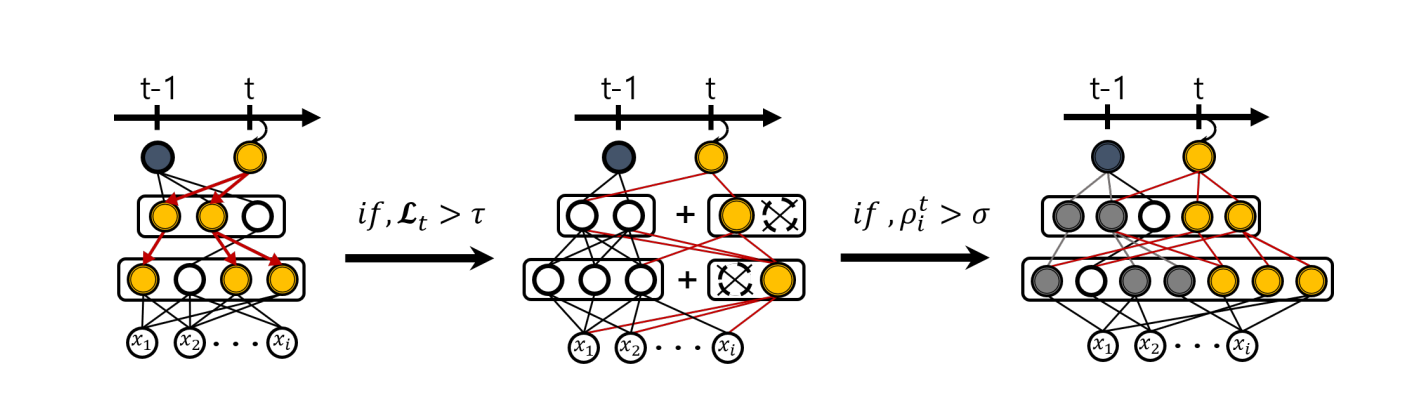
\includegraphics[width=1\linewidth]{figures_ning/den-real}
	\caption[selcted]{expension}
	\label{fig:den-real}
\end{figure}
To address these challenges of lifelong learning, we allow the network to maximize the knowledge gained from previous tasks, while allowing it to dynamically expand its capacity when the accumulated knowledge alone does not adequately explain new tasks. Figure~\ref{fig:den-real} and Algorithm 1 depict our incremental learning process.
\begin{algorithm}[ht]
	\caption{Incremental Learning of a Dynamically Expandable Network}  
	\begin{algorithmic}[1]
		\Require Dataset $\mathcal{D} = (\mathcal{D}_1, \ldots , \mathcal{D}_T )$, Thresholds $\tau,\sigma$
		\Ensure $\bm{W}^T$
		\For{$t=1,\ldots,T$}
		\If{t=1}
		\State Train the network weights $\bm{W}^1$ using Eq.\ref{eq:2}
		\Else
		\State $\bm{W}^t = SelectiveRetraining(\bm{W}^{t-1})$\{Selectively retrain the previous network using Algorithm2\}
		\If{$\mathcal{L}_t>\tau$}
		\State $\bm{W}^t = DynamicExpansion(\bm{W}^{t})$ \{Expand the network capacity using Algorithm3\}
		\EndIf
		\State $\bm{W}^t = Split(\bm{W}^t)$ \{Split and Initialize the units using Algorithm4\}
		\EndIf
		\EndFor
	\end{algorithmic} 
\end{algorithm}

After referring to the research results of others~\cite{yoon2017lifelong}, it was considered that changes should be made in the last step, which is the third step of the algorithm. If the final trained model parameters, i.e., $W$, change relatively large, resulting in the newly trained model no longer being applicable to the old task, they believe that the original nodes should be copied and then retrained~\cite{yoon2017lifelong}. In our experiments, a new approach is taken, where if the model parameters change relatively large, the parameters with large changes are initialized directly after all training is completed, which can satisfy that the newly trained model works well for both the old and new tasks.

In the following subsections, we describe in detail each component of the incremental learning algorithm: 
\begin{itemize}
	\item Selective Retraining
	\item Dynamic Network Expansion
	\item Network Splitting and Initializing
\end{itemize}

\subsection{Selective Retraining}
The easiest way to train a model for a series of tasks is to retrain the entire model each time a new task arrives. However, such retraining would be very expensive for deep neural networks. Therefore, we propose to selectively retrain the model by retraining only the weights affected by the new task. Initially ($t$ = 1), we train the network with $\ell 1$-regularization to promote sparsity of weights so that each neuron is connected to only a few neurons in the following layers:
$$
\underset{\boldsymbol{W}^{t=1}}{\operatorname{minimize}} \mathcal{L}\left(\boldsymbol{W}^{t=1} ; \mathcal{D}_{t}\right)+\mu \sum_{l=1}^{L}\left\|\boldsymbol{W}_{l}^{t=1}\right\|_{1}
\label{eq:2}
$$

Such retraining would be very expensive for deep neural networks. Therefore, we propose to selectively retrain the model by retraining only the weights affected by the new task. Initially (t=1), we train the network with l1-regularization to promote sparsity of the weights so that each neuron is connected to only a few neurons in the following layers.

where $1 \leq l \leq L$ denotes the lth layer of the network, $\boldsymbol{W}_{l}^{t}$ is the network parameter of the lth layer, and $\mu$ is the regularization parameter of the element-wise l1-parametrization of sparsity on $W$ . For the convolutional layer, we apply (2 , 1)-norm on the filters and select only a few filters from the previous layer.
During our incremental learning process, we keep $\boldsymbol{W}^{t-1}$ sparse, so we can significantly reduce the computational overhead if we can focus on new tasks connected to the subnetwork. To this end, when a new task t arrives at the model, we first fit a sparse linear model that predicts the task t using the highest hidden unit of the neural network by solving the following problem:
$$
\underset{\boldsymbol{W}_{L, t}^{t}}{\operatorname{minimize}} \mathcal{L}\left(\boldsymbol{W}_{L, t}^{t} ; \boldsymbol{W}_{1: L-1}^{t-1}, \mathcal{D}_{t}\right)+\mu\left\|\boldsymbol{W}_{L, t}^{t}\right\|_{1}
\label{eq:3}
$$
where $\boldsymbol{W}_{1: L-1}^{t-1}$ denotes the set of all other parameters except $\boldsymbol{W}_{L, t}^{t}$. That is, we solve this optimization to obtain a connection between the output unit ot and the hidden unit in the $L$-1 layer (fixing all other parameters to the $L$-1 layer as $\boldsymbol{W}^{t-1}$). Once we have established sparse connections at this layer, we can identify all the units and weights in the network that are affected by the training, while keeping the parts of the network that are not connected to $o_t$ unchanged. Specifically, we perform a breadth-first search on the network starting from those selected nodes to identify all units (and input features) that have a path to ot. Then, we train only the weights of the selected subnetwork S, denoted as $\boldsymbol{W}_{S}^{t}$:
$$
\underset{\boldsymbol{W}_{S}^{t}}{\operatorname{minimize}} \mathcal{L}\left(\boldsymbol{W}_{S}^{t} ; \boldsymbol{W}_{S^{c}}^{t-1}, \mathcal{D}_{t}\right)+\mu\left\|\boldsymbol{W}_{S}^{t}\right\|_{2}
\label{eq:4}
$$

We use element-by-element $\ell_{2}$-regularizers because sparse connections have already been established. This partial retraining will result in a lower computational overhead and also help to avoid negative migration, since unselected neurons will not be affected by the retraining process. Algorithm~\ref{algorithm:2} describes the selective retraining process:

\begin{algorithm}[ht]
	\caption{Selective Retraining}  
	\begin{algorithmic}[1]
		\Require Dataset $\mathcal{D}_t$, Previous parameter $\bm{W}^{t-1}$
		\Ensure network parameter $\bm{W}^t$
		\State Initialize $l\leftarrow L-1$, $S=\{o_t\}$
		\State Solve Eq.~\ref{eq:3} to obtain $\bm{W}^t_{L,t}$
		\State Add neuron $i$ to $S$ if the weight between $i$ and $o_t$ in $\bm{W}^t_{L,t}$ is not zero.
		\For{$l=L-1,\ldots,1$}
		\State Add neuron $i$ to $S$ if there exists some neuron $j \in S$ such that $\bm{W}^{t-1}_{l,ij}\neq 0$.
		\EndFor
		\State Solve Eq.~\ref{eq:4} to obtain $\bm{W}^t_{S}$
	\end{algorithmic}
	\label{algorithm:2} 
\end{algorithm}

\subsection{Dynamic Network Expansion}
Selective retraining alone is sufficient for the new task if it is highly relevant to the old task or if the aggregated partial knowledge gained from each task is sufficient to explain the new task. However, when the learned features do not accurately represent the new task, additional neurons need to be introduced into the network to take into account the features required for the new task. Some existing works~\cite{rusu2016progressive}are based on a similar idea. However, they are either inefficient due to the need to repeat the iterative training of the forward pass~\cite{zhou2012online} or add a constant number of units in each task t without considering the task difficulty~\cite{rusu2016progressive} and thus are not optimal in terms of performance and network capacity utility.
To overcome these limitations, we propose an efficient approach that uses group sparse regularization to dynamically decide how many neurons to add at which layer for each task without repeatedly retraining the network for each unit. Suppose we extend the $l_{th}$ layer of the network with a constant number of units, say $k$, and introduce two parameter matrix extensions: $\boldsymbol{W}_{l}^{t}=\left[\boldsymbol{W}_{l}^{t-1} ; \boldsymbol{W}_{l}^{\mathcal{N}}\right]$ and $\boldsymbol{W}_{l-1}^{t}=\left[\boldsymbol{W}_{l-1}^{t-1} ; \boldsymbol{W}_{l-1}^{\mathcal{N}}\right]$ for the efferent and afferent layers, where $W^{\mathcal{N}}$ is the extended weight matrix associated with the added neurons. Since we do not always want to add all $k$ units (depending on the correlation between the new and old tasks), we perform group sparse regularization of the added parameters as follows:
$$
\underset{\boldsymbol{W}_{l}^{\mathcal{N}}}{\operatorname{minimize}} \mathcal{L}\left(\boldsymbol{W}_{l}^{\mathcal{N}} ; \boldsymbol{W}_{l}^{t-1}, \mathcal{D}_{t}\right)+\mu\left\|\boldsymbol{W}_{l}^{\mathcal{N}}\right\|_{1}+\gamma \sum_{g}\left\|\boldsymbol{W}_{l, g}^{\mathcal{N}}\right\|_{2}
\label{eq:5}
$$

where $g \in \mathcal{G}$ is the group defined over the incoming weights of each neuron. For the convolutional layer, we define each group as the activation map of each convolutional filter. This group sparse regularization was used by~\cite{wen2016learning} and ~\cite{alvarez2016learning} to find the correct number of neurons for the complete network, while we apply it to parts of the network. Algorithm~\ref{algorithm:3} describes the details of how the extension works.
After selective retraining is completed, the network checks if the loss is below a certain threshold. If not, then at each layer we expand its capacity by $k$ neurons and solve the Eq~\ref{eq:5}. Due to the sparse regularization of the set of Eq.~\cite{eq:5}, the hidden units (or convolutional filters) that are considered unnecessary in the training will be removed completely. We expect that from this dynamic network expansion process, the model captures new features not previously represented by$\boldsymbol{W}_{l}^{t-1}$ to minimize residuals while maximizing the network capacity by avoiding adding too many units.

\begin{algorithm}[h!]
	\caption{Dynamic Network Expansion}  
	\begin{algorithmic}[1]
		\Require Dataset $\mathcal{D}_t$, Threshold $\tau$
		\State Perform Algorithm \ref{label} and compute $\mathcal{L}$
		\If{$\mathcal{L}>\tau$}
		\State Add $k$ units $\bm{h}^\mathcal{N}$ at all layers
		\State Solve for Eq.\ref{label} at all layers
		\EndIf
		\For{$l=L-1,\ldots,1$}
		\State Remove useless units in $\bm{h}^\mathcal{N}_l$
		\EndFor
	\end{algorithmic} 
	\label{algorithm:3}
\end{algorithm}

\subsection{Network Splitting and Initializing}
A key challenge in lifelong learning is the problem of semantic drift or catastrophic forgetting, which describes the problem of a model gradually adapting to a later learned task and consequently forgetting that it learned for an earlier task, leading to a degradation of their performance. The most popular but simplest way to prevent semantic drift is to regularize the parameters so that they do not deviate too much from their original values using $\ell_{2}$-regularization, as follows:
$$
\underset{\boldsymbol{W}^{t}}{\operatorname{minimize}} \mathcal{L}\left(\boldsymbol{W}^{t} ; \mathcal{D}_{t}\right)+\lambda\left\|\boldsymbol{W}^{t}-\boldsymbol{W}^{t-1}\right\|_{2}^{2}
\label{eq:6}
$$

where $t$ is the current task and $\boldsymbol{W}^{t-1}$ is the task {1, . . . , t-1}, and $\lambda$ is the regularization parameter. This $\ell_{2}$-regularization will force the solution Wt to be close to $\boldsymbol{W}^{t-1}$, to the extent given by $\lambda$; if $\lambda$ is small, then the network will learn to reflect the new task more and forget the old task, and if $\lambda$ is large, then $\boldsymbol{W}^{t}$ will retain as much knowledge as possible learned from the previous task. In addition to placing a simple $\ell_{2}$-regularization, each element can be weighted using Fisher information~\cite{kirkpatrick2017overcoming}. Nevertheless, it may be difficult to find a good solution for the previous task and the new task if the number of tasks is large or if the later task is semantically different from the previous one.
In this case, a better solution is to split the neurons so that we have the best features for the two different tasks. In previous studies~\cite{yoon2017lifelong}, the main approach was to replicate the neuron with the larger change after splitting it, so that the original neuron could be left untrained and only the newly added neuron could be trained. However, this method greatly expands the number of neurons, which is not conducive to the retraining of neural networks. We propose a new method: initialization. After executing Eq.~\ref{eq:6}, we measure the semantic drift of each hidden unit $i$, $\rho_{i}^{t}$, as the $\ell_{2}$-distance between $t-1$ and the incoming weights at $t$. Then if $\rho_{i}^{t}>\sigma$, we consider that the meaning of the feature has changed significantly during training, lock this neuron, and initialize it, i.e., the parameter. This operation can be performed in parallel for all hidden units. After this initialization of the neuron, the network does not need to be retrained. This does not change the overall structure, thus increasing the computational effort and memory. Algorithm~\ref{algorithm:4} describes the algorithm for the splitting operation.

\begin{algorithm}[ht]
	\caption{Network Split/Duplication}  
	\begin{algorithmic}[1]
		\Require Weight $\bm{W}^{t-1}$, Threshold $\sigma$
		\State Perform Eq.\ref{label} to obtain $\widetilde{\bm{W}}^t$
		\For{all hidden unit $i$}
		\State $\rho_i^t=\|w_i^t-w_i^{t-1}\|_2$
		\If{$\rho_i^t>\sigma$}
		\State Initialize ${\bm{W}}^t$ into ${\bm{W}}^{t-1}$ 
		\EndIf
		\EndFor
		\State Perform Eq.\ref{label} with the initialization of $\widetilde{\bm{W}}^t$
		to obtain ${\bm{W}}^t$
	\end{algorithmic} 
	\label{algorithm:4}
\end{algorithm}
